\section{Waves}

\begin{multicols}{2}


\section*{Introduction to Waves}


\subsection{String Waves}

\begin{center}
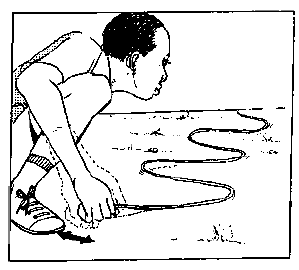
\includegraphics[width=0.4\textwidth]{./img/source/string-waves.png}
\end{center}

\begin{description*}
%\item[Subtopic:]{}
%\item[Materials:]{}
%\item[Setup:]{}
\item[Procedure:]{Take a piece of rope about 6 m long. Hold it at one end and jerk it sideways.}
%\item[Hazards:]{}
\item[Questions:]{Draw a sketch of what you observe.}
%\item[Observations:]{}
\item[Theory:]{The jerking of the rope acts as a source of disturbance which travels along the rope. The direction of motion of the wave is perpendicular to the direction of jerking, so this is a \emph{transverse wave}.}
%\item[Applications:]{}
%\item[Notes:]{}
\end{description*}

\subsection{Flick-Sticks}

\begin{center}
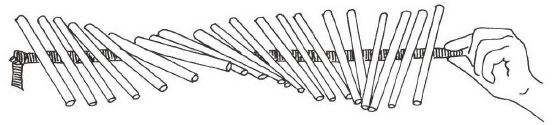
\includegraphics[width=0.49\textwidth]{./img/vso/flick-sticks.jpg}
\end{center}

\begin{description*}
%\item[Subtopic:]{}
\item[Materials:]{Straws or toothpicks, rubber strip or tape, glue}
\item[Setup:]{Cut the straws to be the same length or use toothpicks. Glue them to the tape/rubber strip. A tape of 3 metres works well.}
\item[Procedure:]{Twist or flick the strip to set off waves.}
%\item[Hazards:]{}
%\item[Questions:]{}
%\item[Observations:]{}
%\item[Theory:]{}
%\item[Applications:]{}
\item[Notes:]{Experiment using different lengths of sticks and rubber to create good waves.}
\end{description*}

\subsection{Water Waves}

\begin{center}
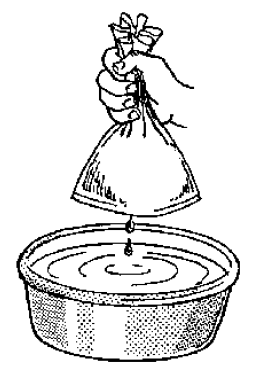
\includegraphics[width=0.25\textwidth]{./img/source/water-waves.png}
\end{center}

\begin{description*}
%\item[Subtopic:]{}
\item[Materials:]{Plastic bag, ink/food colour, water, bucket}
%\item[Setup:]{}
\item[Procedure:]{Use ink or food colour to colour water in a bucket and allow it to come to rest. Fill a plastic bag with water and and poke a small hole in the bottom. Raise the bag so that drops of water fall on the surface of the coloured water.}
%\item[Hazards:]{}
%\item[Questions:]{}
\item[Observations:]{You can see circular waves spreading out rapidly.}
\item[Theory:]{The drops disturb the water. The disturbance spreads out in concentric circles from the centre. These are water waves.}
%\item[Applications:]{}
%\item[Notes:]{}
\end{description*}

\subsection{Energy from Waves}

\begin{center}
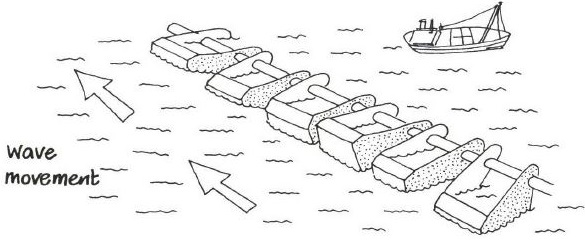
\includegraphics[width=0.45\textwidth]{./img/vso/energy-waves.jpg}
\end{center}

\begin{description*}
%\item[Subtopic:]{}
\item[Materials:]{Stick, floats (wood or card), basin of water}
%\item[Setup:]{}
\item[Procedure:]{Attach several small floats to a long stick as shown. Place in a large basin of water and generate waves with your hand.}
%\item[Hazards:]{}
%\item[Questions:]{}
\item[Observations:]{The floats oscillate up and down on the waves.}
\item[Theory:]{Waves carry energy which can be seen in other objects and converted into electrical energy.}
%\item[Applications:]{}
%\item[Notes:]{}
\end{description*}

\columnbreak

%==================================================================================================%

\section*{Properties of Waves}


\subsection{Water Bottle Sine Wave}

\begin{center}
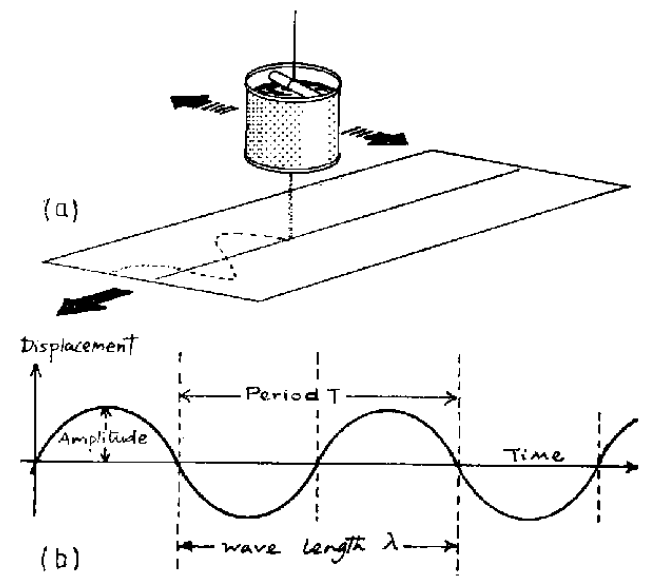
\includegraphics[width=0.4\textwidth]{./img/source/sine-wave.png}
\end{center}

\begin{description*}
%\item[Subtopic:]{}
\item[Materials:]{Water bottle/tin can, pin, coloured water, string}
%\item[Setup:]{}
\item[Procedure:]{Fill a water bottle with water (colour helps to see) and poke a small hole in the cap. Tie a string around the bottle. Walk in a straight line at constant speed while swinging the upside-down bottle from side to side.}
%\item[Hazards:]{}
%\item[Questions:]{}
\item[Observations:]{The pattern produced is a sine wave.}
\item[Theory:]{The oscillation of the bottle spans its \emph{displacement}, while walking at constant speed shows the \emph{time}. Amplitude, wavelength and period may be seen from the wave produced.}
%\item[Applications:]{}
\item[Notes:]{Alternately, suspend an oscillating tin can with a hole in the bottom and slowly pull a long sheet of newspaper at constant speed below it.}
\end{description*}

\subsection{Student Waves}

\begin{center}
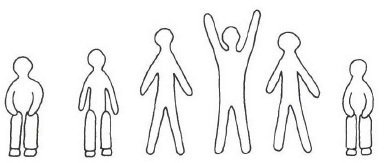
\includegraphics[width=0.4\textwidth]{./img/vso/student-waves.jpg}
\end{center}

\begin{description*}
%\item[Subtopic:]{}
%\item[Materials:]{}
%\item[Setup:]{}
\item[Procedure:]{Students crouch down in a line or circle. One by one in succession, they stand up, making a wave of students.}
%\item[Hazards:]{}
%\item[Questions:]{}
\item[Observations:]{It is not easy to see the wave if you are a part of it!}
\item[Theory:]{The wave carries energy as it passes through the students, but each individual student does not travel with the wave.}
%\item[Applications:]{}
%\item[Notes:]{}
\end{description*}

\subsection{Transfer of Energy}

\begin{center}
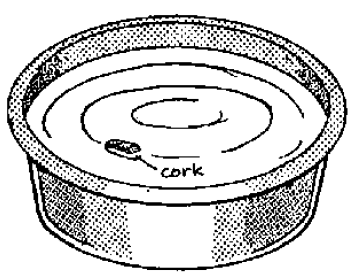
\includegraphics[width=0.35\textwidth]{./img/source/trans-energy.png}
\end{center}

\begin{description*}
%\item[Subtopic:]{}
\item[Materials:]{Small piece of wood/Styrofoam, bowl of water, straw/dropper}
%\item[Setup:]{}
\item[Procedure:]{Put a small piece of wood or Styrofoam on the surface of water in a bowl. With a dropper or straw, release a few drops of water onto the centre of the water surface.}
%\item[Hazards:]{}
%\item[Questions:]{}
\item[Observations:]{The water waves move from the cnetre outwards but the pices of light material do not travel with the wave.}
\item[Theory:]{Energy travels with the wave. However, the particles of the wave-transmitting medium (e.g. water) do \emph{not} travel with the wave, they only oscillate up and down.}
%\item[Applications:]{}
%\item[Notes:]{}
\end{description*}

%==================================================================================================%

\section*{Types of Waves}


\subsection{Slinky Spring}

%\begin{center}
%\includegraphics[width=0.4\textwidth]{./img/source/.png}
%\end{center}

\begin{description*}
%\item[Subtopic:]{}
\item[Materials:]{2 m of flexible steel/copper wire, long rod or stick (3 cm diameter or more)}
\item[Setup:]{Hold one end of the wire against the rod and coil the wire around the cylinder, keeping coils close together.}
\item[Procedure:]{Have a student hold one end of the spring and stretch the slinky slightly so the coils separate. Next, hold the slinky flat on the floor and move one end quickly from side to side while the student holds the other end stationary. Move your hand back and forth, pushing and pulling the spring. Move the slinky to one side then back to the center only once. Observe the waves generated for each case.}
%\item[Hazards:]{}
%\item[Questions:]{}
\item[Observations:]{The transverse wave progresses by alternating crests and troughs, oscillating \emph{perpendicular to the direction of the disturbance}. The longitudinal wave progresses by pushing and pulling \emph{in the direction of the disturbance}. Transverse waves trade crests and troughs when reflected.}
%\item[Theory:]{}
%\item[Applications:]{}
%\item[Notes:]{}
\end{description*}

\subsection{Transverse Pendulum}

\begin{center}
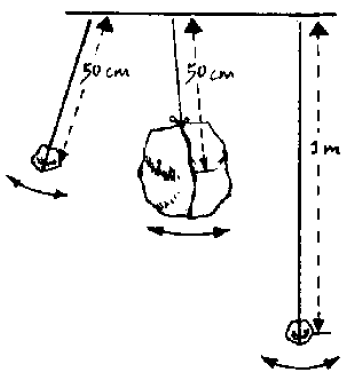
\includegraphics[width=0.4\textwidth]{./img/source/transverse-pendulum.png}
\end{center}

\begin{description*}
%\item[Subtopic:]{}
\item[Materials:]{Stones of different sizes, string}
%\item[Setup:]{}
\item[Procedure:]{Tie a stone to the end of a string 50 cm long. Fix the other end and cause the pendulum to oscillate (no more than 10$^\circ$). Record the time for 20 oscillations and find the frequency (Frequency = number of oscillations $\div$ time). Replace with a heavier stone and repeat. Change the length of string to 100 cm and repeat.}
%\item[Hazards:]{}
%\item[Questions:]{}
\item[Observations:]{The frequency is independent of mass, but depends on the length of the string.}
%\item[Theory:]{}
%\item[Applications:]{}
%\item[Notes:]{}
\end{description*}

\subsection{Longitudinal Pendulum}

\begin{center}
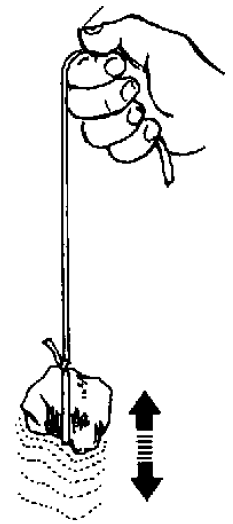
\includegraphics[width=0.15\textwidth]{./img/source/longitudinal-pendulum.png}
\end{center}

\begin{description*}
%\item[Subtopic:]{}
\item[Materials:]{Rubber bands, stones}
%\item[Setup:]{}
\item[Procedure:]{Tie a stone to one end of a rubber band and hold the other end. Lift the stone and release so that it oscillates. Record the time for 20 oscillations and find the frequency. Repeat by varying the length of the rubber band and the mass of the stone.}
%\item[Hazards:]{}
%\item[Questions:]{}
\item[Observations:]{The frequency is independent of mass but depends on length.}
%\item[Theory:]{}
%\item[Applications:]{}
%\item[Notes:]{}
\end{description*}

\subsection{Longitudinal Student Waves}

\begin{center}
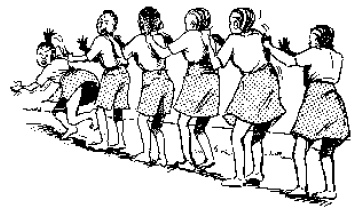
\includegraphics[width=0.45\textwidth]{./img/source/longitudinal-waves.png}
\end{center}

\begin{description*}
%\item[Subtopic:]{}
%\item[Materials:]{}
%\item[Setup:]{}
\item[Procedure:]{Line up a group of students and ask each student to place his/her hands on the shoulder of the student in front. Tell the last student to push forward.}
%\item[Hazards:]{}
%\item[Questions:]{}
\item[Observations:]{A longitudinal wave moves through the queue.}
%\item[Theory:]{}
%\item[Applications:]{}
%\item[Notes:]{}
\end{description*}

%==================================================================================================%

\section*{Behaviour of Waves}


\subsection{Construction of a Ripple Tank}

% Different pic???
\begin{center}
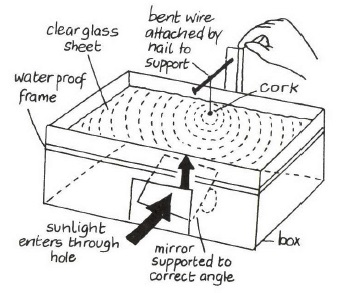
\includegraphics[width=0.49\textwidth]{./img/vso/ripple-tank.jpg}
\end{center}

\begin{description*}
%\item[Subtopic:]{}
\item[Materials:]{Sheet of glass, wooden/plastic/glass strips, waterproof glue, large box, mirror, wooden support, wire, string, small object (e.g. cork or eraser)}
\item[Setup:]{Glue the strips to the glass sheet using waterproof glue to create a shallow glass-bottomed dish. Arrange the mirror in the box so that it can direct light up through the glass and project an image of the ripples on a wall.}
\item[Procedure:]{To create circular waves dip the cork once into the water or tap the support.}
%\item[Hazards:]{}
%\item[Questions:]{}
%\item[Observations:]{}
%\item[Theory:]{}
%\item[Applications:]{}
%\item[Notes:]{}
\end{description*}

\columnbreak

\subsection{Using the Ripple Tank}
\label{sub:rippletank}

%\begin{center}
%\includegraphics[width=0.4\textwidth]{./img/source/.png}
%\end{center}

\begin{description*}
%\item[Subtopic:]{}
\item[Materials:]{Spherical ball, ruler, \nameref{sub:rippletank}, slabs of glass/other barriers}
%\item[Setup:]{}
\item[Procedure:]{Use different objects to observe various behaviours of the waves produced, such as reflection, refraction, diffraction and interference.}
%\item[Hazards:]{}
%\item[Questions:]{}
\item[Observations:]{When a round ball is used, circular waves are produced, while the ruler produces a plane wave. If a barrier is placed in front of the wave, it is reflected back on itself or in a new direction. When passing between two barriers, the wave diffracts and changes form. A plane wave becomes a circular wave and two diffracted waves interfere to form points of constructive and destructive interference.}
%\item[Theory:]{}
%\item[Applications:]{}
%\item[Notes:]{}
\end{description*}

%==================================================================================================%

\section*{Reflection of Waves}


\subsection{Reflection of Water Waves}

\begin{center}
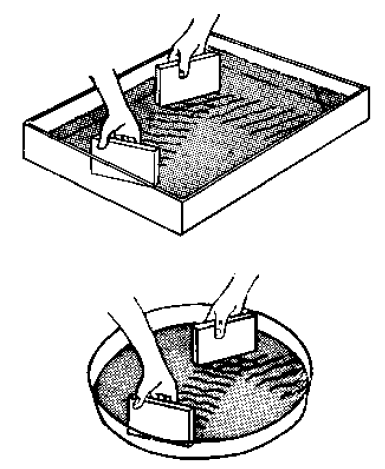
\includegraphics[width=0.4\textwidth]{./img/source/reflection-water-waves.png}
\end{center}

\begin{description*}
%\item[Subtopic:]{}
\item[Materials:]{Large container/dish, coloured water, blocks of wood, plastic/metal}
%\item[Setup:]{}
\item[Procedure:]{Place a straight metal or plastic barrier in the dish containing coloured water. Touch the surface of the water with a rectangular block of wood repeatedly in equal time intervals.}
%\item[Hazards:]{}
%\item[Questions:]{}
\item[Observations:]{Parallel waves move across the dish and rebound from the barrier.}
\item[Theory:]{This behaviour is called \emph{reflection} of the waves. When the angle of the barrier is changed, the angle of reflection remains the same as the angle of incidence.}
\item[Applications:]{The barrier acts as a reflector just as a mirror is a reflector of light.}
%\item[Notes:]{}
\end{description*}

\subsection{Reflection of Sound Waves}

\begin{center}
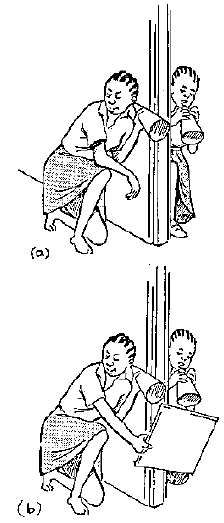
\includegraphics[width=0.4\textwidth]{./img/source/reflection-sound-waves.png}
%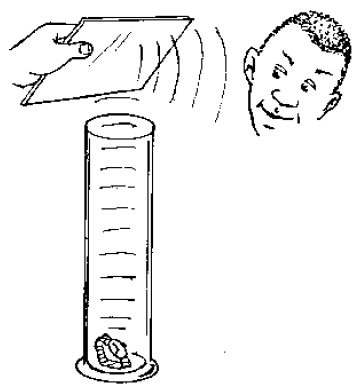
\includegraphics[width=0.4\textwidth]{./img/source/reflection-sound-waves-2.png}
\end{center}

\begin{description*}
%\item[Subtopic:]{}
%\item[Materials:]{}
%\item[Setup:]{}
\item[Procedure:]{2 students stand on either side of a wall. One student whispers into a cone while the other listens through another cone. Repeat while holding a piece of smooth cardboard as shown. Change the position of the cardboard.}
%\item[Hazards:]{}
%\item[Questions:]{}
%\item[Observations:]{}
\item[Theory:]{Initially, no sound is heard. The cardboard reflects the sound waves to the listener, which then allows sound to reach the listener.}
%\item[Applications:]{}
%\item[Notes:]{}
\end{description*}

\columnbreak

\subsection{Reflection in a Rope}

\begin{center}
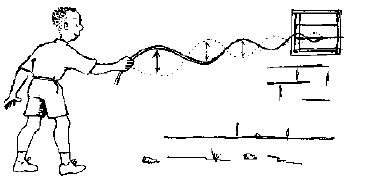
\includegraphics[width=0.45\textwidth]{./img/source/reflection-rope-waves-2.png}
\end{center}

\begin{description*}
%\item[Subtopic:]{}
%\item[Materials:]{}
%\item[Setup:]{}
\item[Procedure:]{Tie a rope about 4 metres long to a fixed bar of a window. Hit the rope with a stick. Repeat by jerking the rope up and down.}
%\item[Hazards:]{}
%\item[Questions:]{}
\item[Observations:]{An impulse travels along the rope and comes back.}
\item[Theory:]{When the impulse hits the fixed end of the rope, it bounces off and comes back as shown by the dotted lines in the figure. The reflected impulse is the same shape as the original, but \emph{inverted}.}
%\item[Applications:]{}
%\item[Notes:]{}
\end{description*}

\subsection{Reflection in a Hose Pipe}

\begin{center}
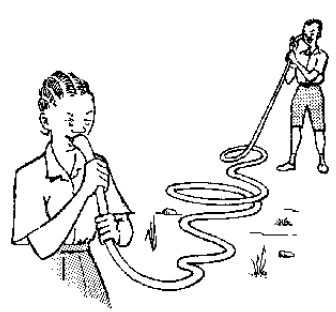
\includegraphics[width=0.4\textwidth]{./img/source/reflection-hose-waves.png}
\end{center}

\begin{description*}
%\item[Subtopic:]{}
%\item[Materials:]{}
%\item[Setup:]{}
\item[Procedure:]{Take a long piece of garden hose pipe. Listen at one end while another person whispers into the other end.}
%\item[Hazards:]{}
%\item[Questions:]{}
\item[Observations:]{The sound is heard more distinctly.}
\item[Theory:]{When a person speaks into the pipe, sound waves are sent into the pipe and reflected off the walls of the hose. These waves are directed to the other end where they can be heard.}
\item[Applications:]{Glass fibres, or fibre optic cables, employ the same principle using light. Light is reflected along the walls of a glass fibre from one end to the other. These cables are used for telephones, televisions, internet cables, etc.}
%\item[Notes:]{}
\end{description*}

%==================================================================================================%

\section*{Sound Waves}


\subsection{Sound from a Ruler}

\begin{center}
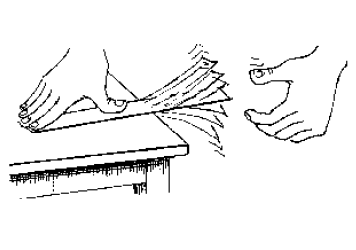
\includegraphics[width=0.4\textwidth]{./img/source/sound-ruler.png}
\end{center}

\begin{description*}
%\item[Subtopic:]{}
%\item[Materials:]{}
%\item[Setup:]{}
\item[Procedure:]{Tightly hold a ruler on a table with its free end extending over the edge. Cause the free end to vibrate and listen to the sound. Repeat for different extending lengths of the ruler.}
%\item[Hazards:]{}
\item[Questions:]{How does the sound change with extending length of the ruler?}
\item[Observations:]{When the vibrating length is reduced, a higher pitch and quieter sound is heard and the vibrations become faster and faster. When the vibrating length is increased, a lower pitch and louder sound is heard.}
\item[Theory:]{The short lengths cause small masses of air to vibrate with small amplitudes and so produce a soft sound. The long lengths vibrate large masses of air with large amplitudes, making a louder sound.}
%\item[Applications:]{}
%\item[Notes:]{}
\end{description*}

\subsection{Straw Kazoo}

%\begin{center}
%\includegraphics[width=0.4\textwidth]{./img/source/.png}
%\end{center}

\begin{description*}
%\item[Subtopic:]{}
\item[Materials:]{Straw, scissors}
%\item[Setup:]{}
\item[Procedure:]{Cut one end of a straw so that it comes to a point like an arrowhead. Blow into the straw to produce a sound like a kazoo or vuvuzela. While blowing, cut short lengths of the free end of the straw continually until it is very short.}
%\item[Hazards:]{}
%\item[Questions:]{}
\item[Observations:]{As you cut off lengths of the straw, the sound produced becomes a higher pitch.}
\item[Theory:]{Vibrations in the long straw have a low frequency and hence low pitch, while those in the short straw have a high frequency and hence high pitch.}
%\item[Applications:]{}
%\item[Notes:]{}
\end{description*}

\columnbreak

\subsection{Sound Sandwich}

\begin{center}
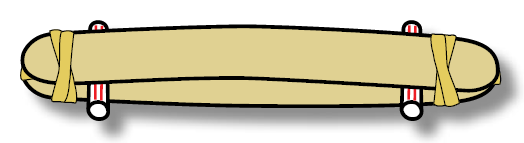
\includegraphics[width=0.4\textwidth]{./img/sound-sandwich.jpg}
\end{center}

\begin{description*}
%\item[Subtopic:]{}
\item[Materials:]{Straw, scissors, 2 tongue depressors, 2 small rubber bands, 1 wide rubber band}
\item[Setup:]{Stretch a wide rubber band lengthwise across a tongue depressor. Cut two small pieces of straw (about 3 cm) and place them under the rubber band about a third of the way from either end. Cover with the other tongue depressor and fix the two together at the ends with the small rubber bands.}
\item[Procedure:]{Blow through the sticks (not the straws) to hear a sound. Change the position of the straws and blow again.}
%\item[Hazards:]{}
%\item[Questions:]{}
%\item[Observations:]{}
\item[Theory:]{The sound produced is caused by vibrations in the wide rubber band. The pitch depends on the length of rubber band between the two straws. A longer length produces a lower pitch, while a shorter length produces a higher pitch.}
%\item[Applications:]{}
%\item[Notes:]{}
\end{description*}

\subsection{Sound Vibrations}

\begin{center}
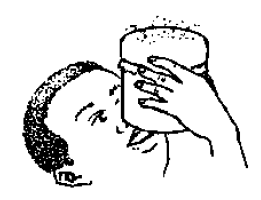
\includegraphics[width=0.4\textwidth]{./img/source/sound-vibrations.png}
\end{center}

\begin{description*}
%\item[Subtopic:]{}
\item[Materials:]{Open tin, paper, rubber band, sand}
%\item[Setup:]{}
\item[Procedure:]{Cover a one end of an open tin with a membrane (paper) and fasten it using a rubber band. Spread fine dry sand on the membrane. Speak a soft and loud sound into the tin from the bottom while a friend watches the sand.}
%\item[Hazards:]{}
%\item[Questions:]{}
\item[Observations:]{The louder the sound, the larger the amplitude of the vibrations.}
\item[Theory:]{The air underneath the membrane gets disturbed by the sound waves which in turn disturb the membrane and make it vibrate. This shows that sound travels as a vibration.}
%\item[Applications:]{}
%\item[Notes:]{}
\end{description*}

\columnbreak

\subsection{Drum Vibrations}

\begin{center}
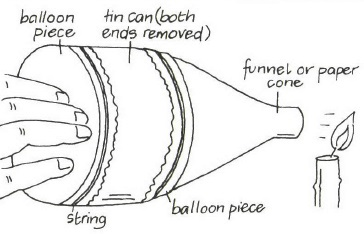
\includegraphics[width=0.45\textwidth]{./img/vso/drum-vibrations.jpg}
\end{center}

\begin{description*}
%\item[Subtopic:]{}
\item[Materials:]{Tin can, balloon, string, funnel, candle}
\item[Setup:]{Remove the ends from the tin. Tie the balloon pieces to the tin as shown and attach the funnel.}
\item[Procedure:]{Place the drum in front of a lit candle and tap the drum softly and then harder.}
%\item[Hazards:]{}
%\item[Questions:]{}
\item[Observations:]{When the drum is tapped hard, it can put out the candle.}
\item[Theory:]{Sound vibrations are carried through the air in the can, making the other sheet vibrate. The funnel concentrates the sound vibrations so that the air from the funnel can put out the candle.}
%\item[Applications:]{}
%\item[Notes:]{}
\end{description*}

\subsection{Knocking a Water Tank}

\begin{center}
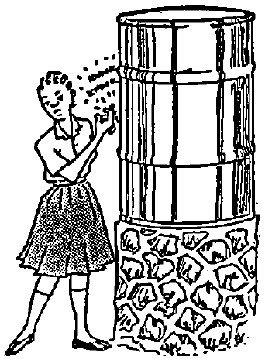
\includegraphics[width=0.32\textwidth]{./img/source/knocking-water-tank.png}
\end{center}

\begin{description*}
%\item[Subtopic:]{}
%\item[Materials:]{}
%\item[Setup:]{}
\item[Procedure:]{Gently knock the side of a water tank from the top downwards to the bottom and listen to the tones.}
%\item[Hazards:]{}
%\item[Questions:]{}
\item[Observations:]{A loud sound is heard at the top, and a soft sound at the bottom.}
\item[Theory:]{The knock causes the drum to vibrate. At the top, the knocking vibrates the air inside the tank giving a loud sound. At the bottom, the knocking vibrates water inside the tank giving a soft sound.}
\item[Applications:]{This can be used to check the presence of liquids in tanks or large containers.}
%\item[Notes:]{}
\end{description*}

%==================================================================================================%

\section*{Propagation of Sound Waves}
%Sound does not travel through a vacuum. It requires a \emph{medium} for its propagation. Denser media are better transmitters of sound than less dense media. Thus, sound travels faster and better in water, wood or strings than in air.


\subsection{String Telephone}

\begin{center}
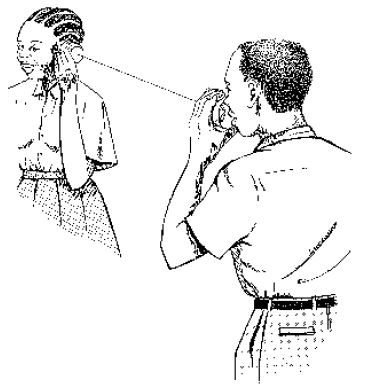
\includegraphics[width=0.4\textwidth]{./img/source/wave-motion.jpg}
\end{center}

\begin{description*}
%\item[Subtopic:]{}
\item[Materials:]{2 tin cans, string}
%\item[Setup:]{}
\item[Procedure:]{Punch a small hole at the centre of the bottom of each empty can. Connect the cans with a long string knotted inside each can. Hold the cans so that the string is stretched. One student talks into one can while another listens through the other can.}
%\item[Hazards:]{}
%\item[Questions:]{}
\item[Observations:]{The speaker can be heard distinctly, even with the other ear closed with a finger.}
\item[Theory:]{Sound travels through the string (as a medium) from one can to the other.}
%\item[Applications:]{}
%\item[Notes:]{}
\end{description*}

\subsection{Sound in Air}

\begin{center}
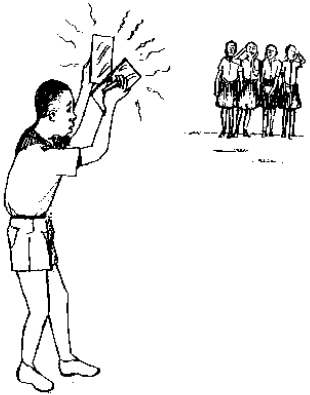
\includegraphics[width=0.35\textwidth]{./img/source/sound-in-air.png}
\end{center}

\begin{description*}
%\item[Subtopic:]{}
%\item[Materials:]{}
%\item[Setup:]{}
\item[Procedure:]{One student stands about 100 m from the class and makes sound by clapping two metal lids together.}
%\item[Hazards:]{}
%\item[Questions:]{}
%\item[Observations:]{}
\item[Theory:]{The sound is transmitted from the source to the class using air as a medium.}
%\item[Applications:]{}
%\item[Notes:]{}
\end{description*}

\subsection{Sound in a String}

\begin{center}
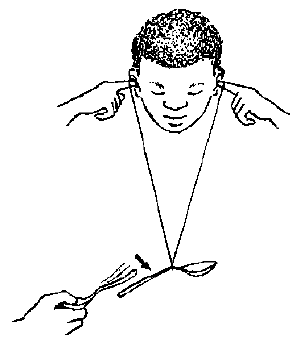
\includegraphics[width=0.4\textwidth]{./img/source/sound-in-string.png}
\end{center}

\begin{description*}
%\item[Subtopic:]{}
\item[Materials:]{Thread, 2 spoons}
%\item[Setup:]{}
\item[Procedure:]{Tie a metal spoon at the middle of a 1 m cotton thread. Wind each end of the thread around a fingertip and press the fingertips into your ears. Bend down so the spoon hangs freely and let someone hit the spoon slightly with a nail or another spoon.}
%\item[Hazards:]{}
%\item[Questions:]{}
\item[Observations:]{A chime is heard like that of a church bell.}
\item[Theory:]{Sound travels through the string to your ears. Sound travels better in strings than in air.}
%\item[Applications:]{}
%\item[Notes:]{}
\end{description*}

\subsection{Sound in Wood}

\begin{center}
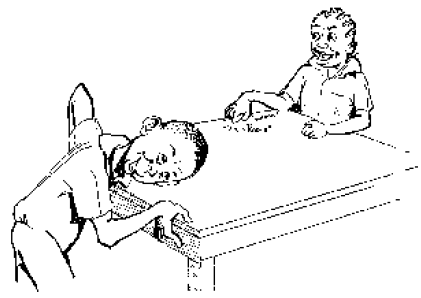
\includegraphics[width=0.45\textwidth]{./img/source/sound-in-wood.png}
\end{center}

\begin{description*}
%\item[Subtopic:]{}
%\item[Materials:]{}
%\item[Setup:]{}
\item[Procedure:]{Place your ear against one edge of a table while a friend is knocking the opposite edge slightly. Listen to the sound through air and the sound through the table.}
%\item[Hazards:]{}
%\item[Questions:]{}
\item[Observations:]{The sound traveling through the table is heard more distinctly than when heard through the air.}
\item[Theory:]{Sound travels better in wood than in air.}
%\item[Applications:]{}
%\item[Notes:]{}
\end{description*}

\subsection{Sound in Metal}

\begin{center}
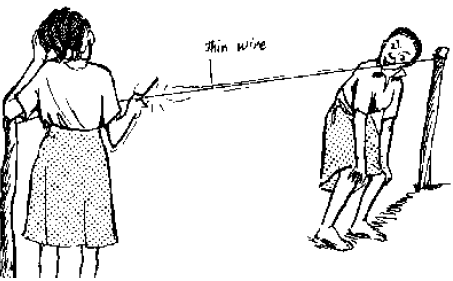
\includegraphics[width=0.49\textwidth]{./img/source/sound-in-metal.png}
\end{center}

\begin{description*}
%\item[Subtopic:]{}
%\item[Materials:]{}
%\item[Setup:]{}
\item[Procedure:]{Fix a long thin wire to two posts about 5 m apart. One student scratches the wire while the other listens both in air and by placing an ear against the wire.}
%\item[Hazards:]{}
%\item[Questions:]{}
\item[Observations:]{Nothing is heard unless the student's ear is placed against the wire.}
\item[Theory:]{Sound travels better in metal than it does in air.}
%\item[Applications:]{}
%\item[Notes:]{}
\end{description*}

\subsection{Sound in Water}

\begin{center}
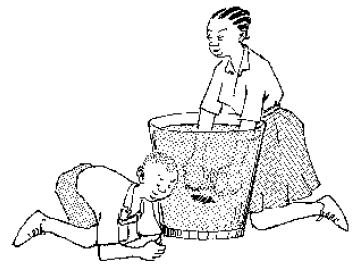
\includegraphics[width=0.45\textwidth]{./img/source/sound-in-water.png}
\end{center}

\begin{description*}
%\item[Subtopic:]{}
\item[Materials:]{Plastic bucket, water, 2 stones}
%\item[Setup:]{}
\item[Procedure:]{Fill a plastic bucket with water and knock 2 stones against each other \emph{in the water} while another person puts an ear close to the bucket.}
%\item[Hazards:]{}
%\item[Questions:]{}
\item[Observations:]{The sound is heard more loudly when listening near the bucket.}
\item[Theory:]{Sound travels better in water than in air.}
%\item[Applications:]{}
%\item[Notes:]{}
\end{description*}

\columnbreak

\subsection{Doppler Whirl}

%\begin{center}
%\includegraphics[width=0.4\textwidth]{./img/source/.png}
%\end{center}

\begin{description*}
%\item[Subtopic:]{}
\item[Materials:]{Mobile phone, sock, string}
%\item[Setup:]{}
\item[Procedure:]{Program a ring tone on a mobile phone that repeats a single note for a period of 20 seconds or more. Place the phone in a sock, tie it to a string and swing it rapidly around your head so that the phone moves in a large circle.}
%\item[Hazards:]{}
%\item[Questions:]{}
\item[Observations:]{As the phone moves towards the students, they will hear the pitch increased, and as it moves away, they will hear the pitch decreased. The person swinging the phone hears no noticeable difference in pitch.}
\item[Theory:]{This is known as the Doppler effect. When the source of a sound is moving, the sound waves in front of the source become compressed, making for shorter wavelengths and higher frequency. The sound waves behind the source are extended (like they are being stretched), so the wavelength is longer and frequency lower.}
\item[Applications:]{The same effect is seen for sirens of an ambulance or emergency vehicle approaching and moving away from you.}
%\item[Notes:]{}
\end{description*}

%==================================================================================================%

\section*{Musical Instruments}


\subsection{Bottle Orchestra}

\begin{center}
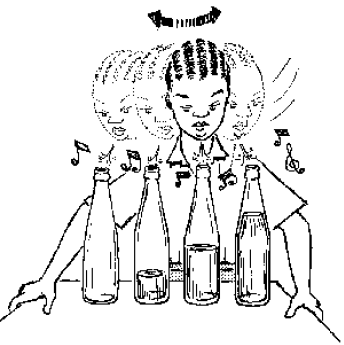
\includegraphics[width=0.45\textwidth]{./img/source/bottle-orchestra.png}
\end{center}

\begin{description*}
%\item[Subtopic:]{}
\item[Materials:]{4 bottles, water}
%\item[Setup:]{}
\item[Procedure:]{Fill four equal bottles with different levels of water and blow into the bottles one after another, listening to the tones produces.}
%\item[Hazards:]{}
%\item[Questions:]{}
\item[Observations:]{The shorter the air column, the higher the tones.}
\item[Theory:]{Adding water shortens the height of the column of air, shortening the wavelength and increasing the frequency.}
\item[Applications:]{Organ, flute}
%\item[Notes:]{}
\end{description*}

\columnbreak

\subsection{Bamboo Organ}

\begin{center}
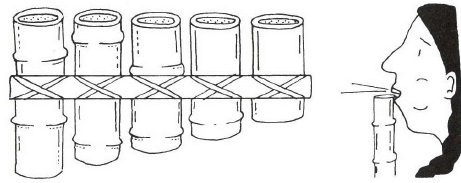
\includegraphics[width=0.45\textwidth]{./img/vso/bamboo-organ.jpg}
\end{center}

\begin{description*}
%\item[Subtopic:]{}
\item[Materials:]{Pieces of bamboo, string/tape}
%\item[Setup:]{}
\item[Procedure:]{Hollow out the bamboo pieces and attach them as shown. The length of the pipes determines the pitch of the sound.}
%\item[Hazards:]{}
%\item[Questions:]{}
%\item[Observations:]{}
%\item[Theory:]{}
%\item[Applications:]{}
%\item[Notes:]{}
\end{description*}

\subsection{Bamboo Flute}

\begin{center}
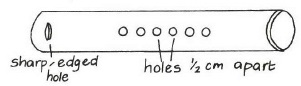
\includegraphics[width=0.45\textwidth]{./img/vso/bamboo-flute.jpg}
\end{center}

\begin{description*}
%\item[Subtopic:]{}
\item[Materials:]{Bamboo tube (1.5 cm diameter, 30 cm length)}
%\item[Setup:]{}
\item[Procedure:]{Hollow out the bamboo tube and dry it until its colour changes to yellowish-brown. Make a mouth-piece and row of holes as shown. Blow air into the mouth-piece while closing some of the holes with your fingers.}
%\item[Hazards:]{}
%\item[Questions:]{}
\item[Observations:]{Different tones are produced by the flute as you remove your fingers from different holes.}
\item[Theory:]{The pitch of the tones depends on the distance of the first open hole from the mouth-piece, i.e. the closer the whole hole is to the mouth-piece, the higher the tone produced. Thus the tone produced is determined by the vibration of air in the column between the mouth-piece and the first uncovered hole.}
%\item[Applications:]{}
%\item[Notes:]{}
\end{description*}

\columnbreak

\subsection{Marimba}

\begin{center}
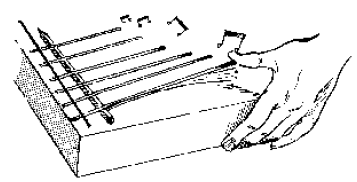
\includegraphics[width=0.4\textwidth]{./img/source/marimba.png}
\end{center}

\begin{description*}
%\item[Subtopic:]{}
\item[Materials:]{Bicycle spokes, piece of wood, pencil}
\item[Setup:]{Cut bicycle spokes into different lengths and arrange them on a piece of wood. Fix them with another spoke across as shown. Lift the spokes by inserting a pencil underneath them.}
\item[Procedure:]{Pluck the free ends one after another and listen to the tones produced.}
%\item[Hazards:]{}
%\item[Questions:]{}
%\item[Observations:]{}
\item[Theory:]{Plucking causes the spokes to vibrate and produce sound. The longer the spoke, the lower the tone.}
%\item[Applications:]{}
%\item[Notes:]{}
\end{description*}

\subsection{Xylophone}

\begin{center}
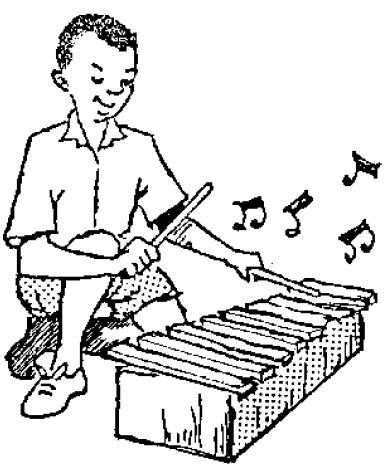
\includegraphics[width=0.4\textwidth]{./img/source/xylophone.png}
\end{center}

\begin{description*}
%\item[Subtopic:]{}
\item[Materials:]{Wooden box, wooden bars, string, sticks}
%\item[Setup:]{}
\item[Procedure:]{Make a wooden box with the bottom and top sides open. Take timber bars of different types and thickness. Drill four holes into each bar and pass two strings to hold all the bars together on the top of the wooden box. Beat the bars in turn using two sticks.}
%\item[Hazards:]{}
%\item[Questions:]{}
\item[Observations:]{Different sizes of bars give different tones and different materials of the same thickness give different tones.}
%\item[Theory:]{}
%\item[Applications:]{}
%\item[Notes:]{}
\end{description*}

%==================================================================================================%

\section*{Stationary Waves}


\subsection[Sonometer (One-String Guitar)]{Sonometer (One-String \hfill \\ Guitar)}

\begin{center}
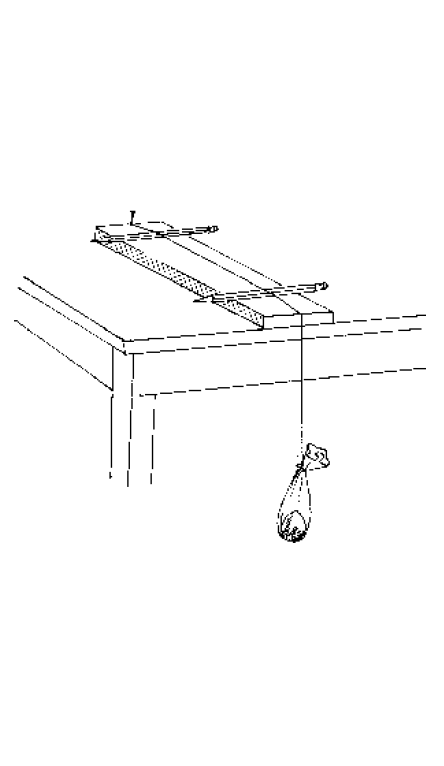
\includegraphics[width=0.4\textwidth]{./img/source/sonometer.png}
\end{center}

\begin{description*}
%\item[Subtopic:]{}
\item[Materials:]{Soft wood board, string or thin wire, nail, plastic bag, stones, 2 pencils}
\item[Setup:]{Place a soft board on a table. Fix a string with a nail to one end of the soft board and tie a heavy mass of stones to the other end so that it hangs below the edge of the table. Insert two pencils under the thread so as to raise the thread off the board.}
\item[Procedure:]{Pluck the thread between the two pencils. Repeat by varying the distance between the pencils and the mass hanging.}
%\item[Hazards:]{}
%\item[Questions:]{}
\item[Observations:]{Reducing the distance between the pencils produces a higher tone. Increasing the mass produces a higher tone.}
\item[Theory:]{The tone produced by the vibrating string depends on its vibrating length and the tension in the string.}
%\item[Applications:]{}
%\item[Notes:]{}
\end{description*}

\vfill
\columnbreak

\subsection{Resonance Tube}

\begin{center}
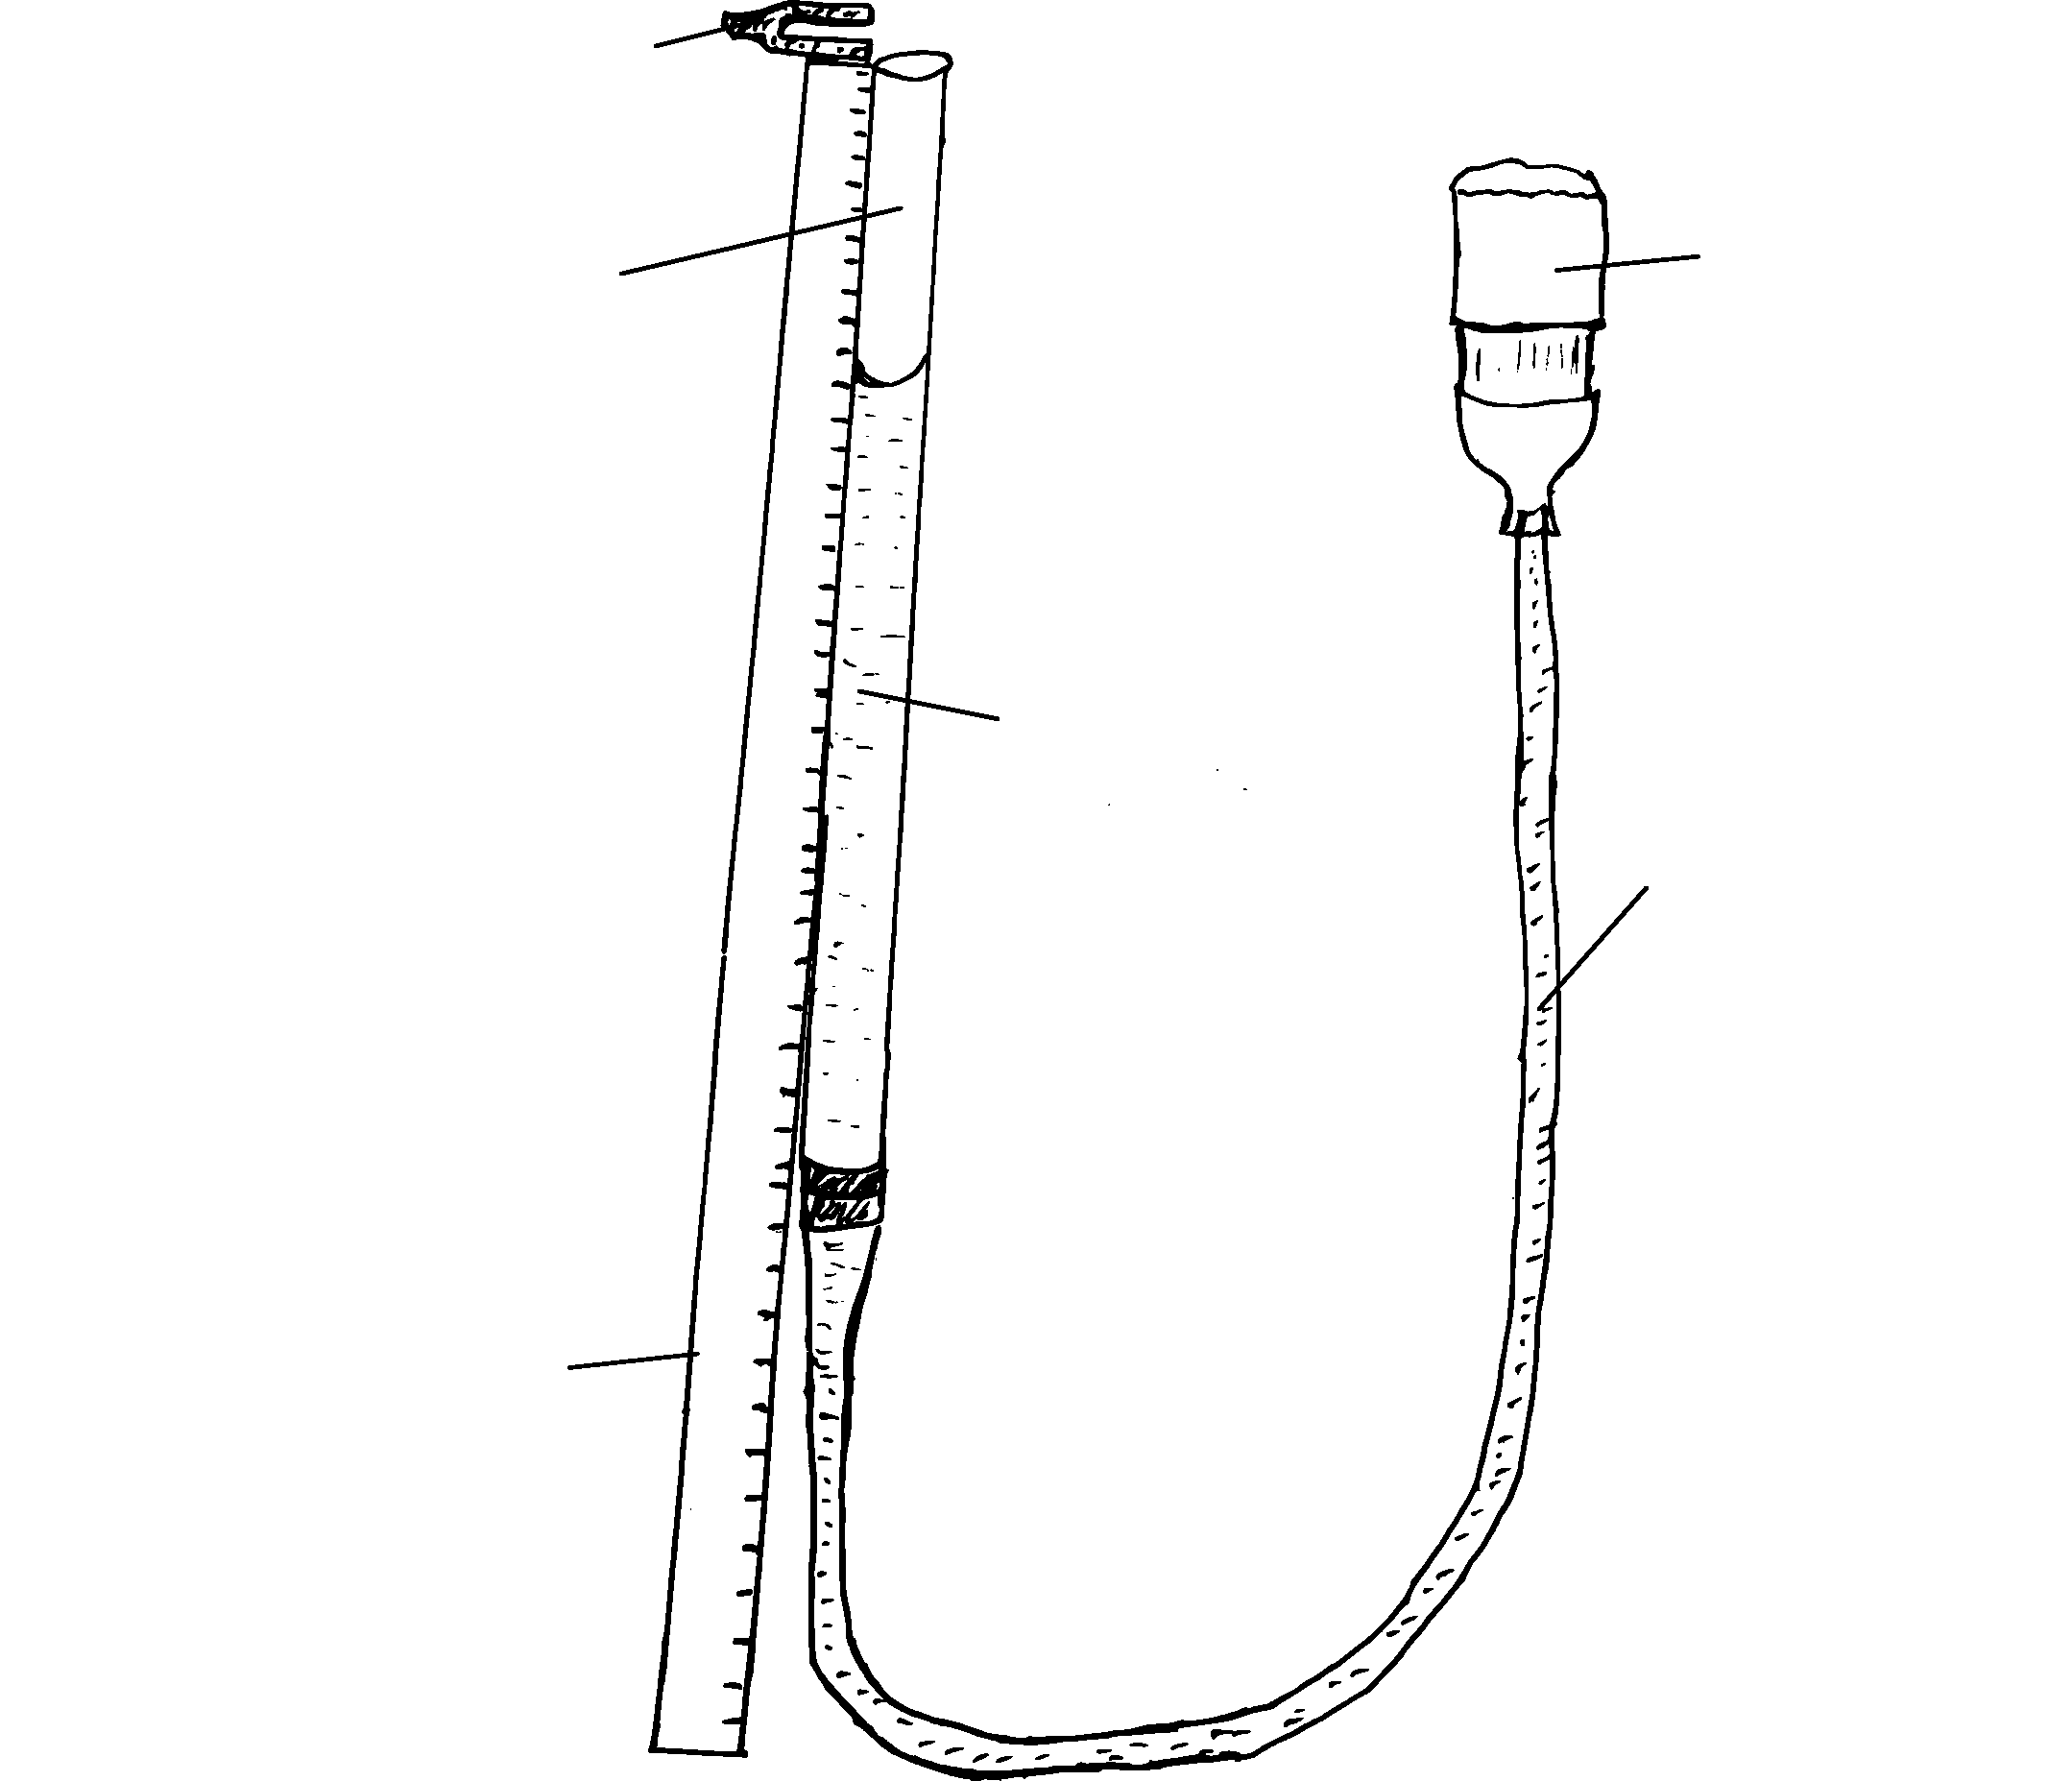
\includegraphics[width=0.49\textwidth]{./img/resonance-tube.png}
\end{center}

\begin{description*}
%\item[Subtopic:]{}
\item[Materials:]{Fluorescent tube (tube light), thick rubber tubing, two 1.5 L plastic water bottles, super glue, wax, turning fork, retort stand, bucket, water, long stick, knife, metre rule, rubber or cork, piece of cloth}
\item[Setup:]{Carefully cut the rims off both sides of the tube and clean it with a cloth on a long stick. Cut the bottom 5 cm off one bottle (bottle 1) and the top 5 cm off the other (bottle 2). Make a hole in each bottle cap and insert the rubber tubing through both holes. Attach one end of the pipe with glue and wax to the inside top of bottle 2. Hold the tube vertically with a metre rule using a retort stand. Raise bottle 1 vertically until you have created a U-shape and pour water into bottle 1.}
\item[Hazards:]{Do not touch the fluorescent dust in the tube; it is poisonous.}
\item[Procedure:]{Strike the tuning fork with a soft material (e.g. rubber) and place it at the top of the tube. Raise and lower the water level in the tube by changing the vertical position of bottle 1. Repeat for different tuning forks, noting the fundamental note and overtone.}
%\item[Questions:]{}
\item[Observations:]{The tube can be heard resonating at two or more water levels. The lowest water level is the fundamental and each smaller water level is a higher harmonic.}
\item[Theory:]{The length of the tube from the water to the top can be used to calculate the speed of sound in air. Resonance frequency occurs when the natural frequency of the air column is equal to the forced frequency from the tuning fork.}
%\item[Applications:]{}
%\item[Notes:]{}
\end{description*}

%==================================================================================================%


%\subsection{Speed of Sound in Air}
%
%%\begin{center}
%%\includegraphics[width=0.4\textwidth]{./img/source/.png}
%%\end{center}
%
%\begin{description*}
%%\item[Subtopic:]{}
%\item[Materials:]{}
%\item[Setup:]{}
%\item[Procedure:]{}
%\item[Hazards:]{}
%\item[Questions:]{}
%\item[Observations:]{}
%\item[Theory:]{}
%\item[Applications:]{}
%\item[Notes:]{}
%\end{description*}

\end{multicols}

\pagebreak